%%%%%%%%%%%%%%%%%%%%%% Props %%%%%%%%%%%%%%%%%%%%%%
\documentclass{article}

\usepackage[french]{babel}
\usepackage[utf8]{inputenc}
\usepackage[T1]{fontenc}
\usepackage{graphicx}
\usepackage{fancyhdr}
\usepackage{eurosym}
\usepackage{color}
\usepackage{soul}
\usepackage{listings}
\usepackage{enumitem}
\usepackage{enumerate}

\pagestyle{fancy}
\lhead{Soutenance 3}
\chead{Deadly Science}
\rhead{Custos Carceris}

\definecolor{mygreen}{rgb}{0,0.6,0}
\definecolor{mygray}{rgb}{0.5,0.5,0.5}
\definecolor{mymauve}{rgb}{0.58,0,0.82}

\lstset{ 
  commentstyle=\color{mygreen},
  keywordstyle=\color{blue},       % keyword style
  numberstyle=\tiny\color{mygray}, % the style that is used for the line-numbers
  rulecolor=\color{black},         % if not set, the frame-color may be changed on line-breaks within not-black text (e.g. comments (green here))
  stringstyle=\color{mymauve},     % string literal style
  language=[Sharp]C,                 % the language of the code
  backgroundcolor=\color{white},   % choose the background color; you must add \usepackage{color} or \usepackage{xcolor}; should come as last argument
  basicstyle=\footnotesize,        % the size of the fonts that are used for the code
  breakatwhitespace=true,         % sets if automatic breaks should only happen at whitespace
  breaklines=true,
  extendedchars=true,              % lets you use non-ASCII characters; for 8-bits encodings only, does not work with UTF-8
  frame=single,	                   % adds a frame around the code
  tabsize=2,	                   % sets default tabsize to 2 spaces
  showstringspaces=false,
  numbers=left,
}

\begin{document}


%%%%%%%%%%%%%%%%%%%%%% Titre %%%%%%%%%%%%%%%%%%%%%%
\begin{titlepage}
	\centering
	{\scshape\LARGE Custos Carceris\par}
	\vspace{1cm}
	{\scshape\Large Rapport de projet\par}
	\vspace{1.5cm}
	{\huge\bfseries Deadly Science\par}
	\vspace{2cm}
	
\includegraphics[width=0.5\textwidth]{logo.png}\par\vspace{1cm}
	{\Large\itshape Léandre Perrot\par}
	{\Large\itshape Yann Boudry\par}
	{\Large\itshape Steve Suissa\par}
	{\Large\itshape Célian Raimbault\par}
	\vfill
	Un projet EPITA
	\vfill
	{\large \today\par}
\end{titlepage}



\newpage
\tableofcontents


%%%%%%%%%%%%%%%%%%%%% Intro %%%%%%%%%%%%%%%%%%%%%%

\newpage
\section{Introduction}

%%%%%%%%%%%%%%% TODO : Mettre a jour
Le jeu a grandement avancé depuis le retour du cahier des charges : le réseau est quasiment entièrement fonctionnel, pareil pour la caméra, le site avance petit à petit, la génération est presque fini et certaines musiques ont été composées. Globalement, le jeu est quasiment jouable.
\begin{table}[!h]
\centering
\caption{Avancement}
\begin{tabular}{|l|l|l|}

\hline
%%%%%%%%%%%%%%% TODO : Mettre a jour
Tâches $\backslash$Soutenances & Attendu & Réalité \\ \hline
Camera & 50\% & 75\% \\ \hline
G Joueur & 30\% & 50\% \\ \hline
G Jeu & 30\% & 30\% \\ \hline
Reseau & 50\% & 75\% \\ \hline
Map Const & 30\% & 30\% \\ \hline
Menu & 15\% & 70\% \\ \hline
Chrono/GUI & 30\% & 30\% \\ \hline
Site TXT & 0\% & 30\% \\ \hline
Site E & 0\% & 0\% \\ \hline
Map Gen & 0\% & 50\% \\ \hline
Musique & 0\% & 25\% \\ \hline
Sons & 0\% & 10\% \\ \hline

\end{tabular}
\end{table}
 
\newpage
\section{Reprise du cahier des charges}
blablabla
\newpage
\section{Présentation du projet}



\subsection{Menus}
blablabla
%%%%%%%%%%%%%%%%%%%%%% Yann %%%%%%%%%%%%%%%%%%%%%%%%%%%%%%
\subsubsection{Menu principal}
blablabla
\newpage
\subsubsection{Menus de connection}
%%%%%%%%%%%%%%%%%%%%%% Steve%%%%%%%%%%%%%%%%%%%%%%%%%%%%%%
Pour se connecter il y'a trois menus, le menu pour créer la partie, le menu pour changer les paramètres de la partie, et enfin le menu on peut voir les joueurs connectés et commencer la partie. Chacun des 3 menus ont subi une refonte graphique pour correspondre à l'ambiance du jeu et avoir un aspect visuel plus plaisant.

\paragraph{Menu pour créer la partie}

Voici à quoi ce menu ressemble : 

\begin{figure}[!ht]
    \centering
    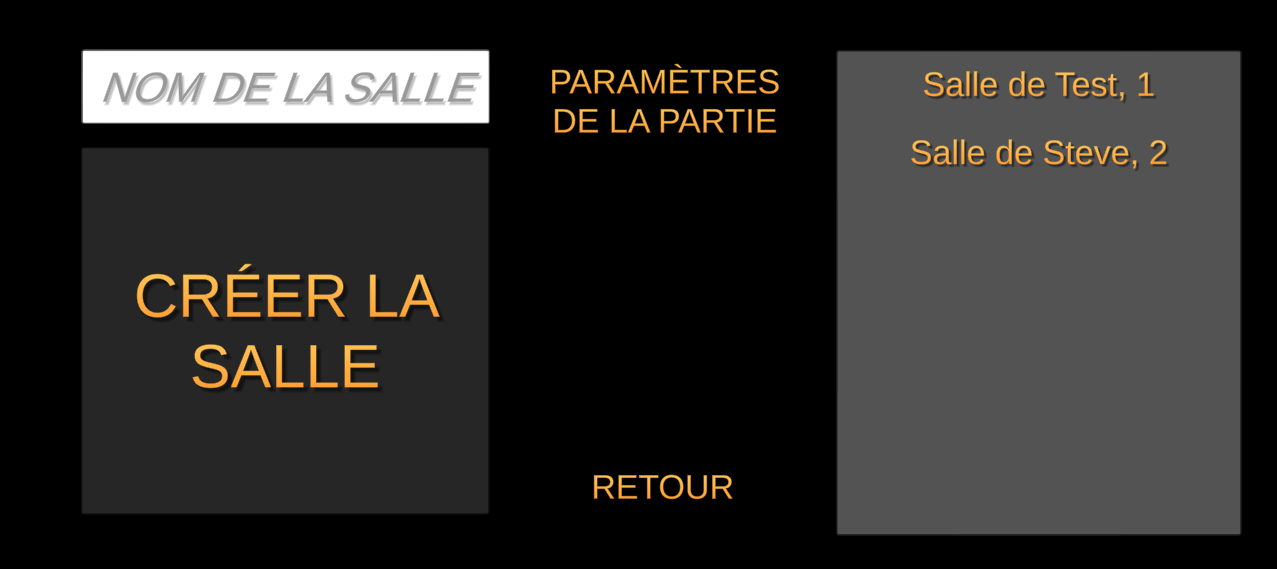
\includegraphics[width=0.8\textwidth]{Menu1.png}
    \caption{Menu pour créer la salle}
    \label{Menu pour créer la salle}
\end{figure}

Il est composé de deux parties. Celle de gauche on peut écrire dans la barre blanche le nom de la salle que l'on veut créer et un bouton "Créer la salle" qui comme son nom l'indique permet de créer la salle et d'entrer dans un autre menu que l'on verra par la suite. La partie droite liste chacune des salles avec leur noms et le nombre de joueurs déjà présents dans la salle. Elle est sur un tableau défilant ce qui permet d'avoir autant de parties que l'on souhaite. Cela permet de savoir si par exemple on va attendre plus ou moins longtemps avant le début de la partie. Pour rejoindre la salle que l'on souhaite, c'est simple, il suffit de cliquer dessus et cela nous fait rentrer dans la dite salle. A noter que si la salle est remplie à son maximum, elle ne sera pas montrée comme visible, vu qu'on ne peut pas la rejoindre. En ce qui concerne les deux boutons du milieu, le bouton "Retour" nous fait retourner à l'écran principal et le deuxième bouton nous transporte dans le menu des paramètres du labyrinthe que l'on va maintenant regarder.

\paragraph{Menu pour les paramètres de la partie}

Dans ce menu on peut changer de mode de jeu entre Classique et Nocturne (ces modes de jeu seront expliqués par la suite). On peut aussi changer le nombre de joueurs de la partie. Enfin on peut choisir la taille du labyrinthe parmis plusieurs dimensions prédéfinies ou bien choisir une taille personnalisée (par exemple un labyrinthe rectangulaire) en l'écrivant sur la barre blanche et confirmer. Pour sélectionner l'option que l'on souhaite, il suffit encore tout simplement de cliquer dessus. Par exemple sur la Figure 2, on peut voir que le mode de jeu choisi est Classique, que la salle peut contenir quatre joueurs et que la taille du labyrinthe est de dix en largeur et 10 en longueur. Lorsque l'on a choisi ses paramètres, il suffit d'appuyer sur le bouton "Retour" qui nous envoie sur le menu précédant et on peut créer la partie avec les paramètres enregistrés. On peut souligner que les modes de jeu et les tailles du labyrinthe sont sur des tableaux défilants, ce qui permet premièrement l'ajout de nouveaux modes ou de nouvelles tailles facile, mais aussi que l'on peut en ajouter autant qu'on veut, il suffit juste d'utiliser la molette de la sourie pour accéder aux options tout en bas.



\begin{figure}[!ht]
    \centering
    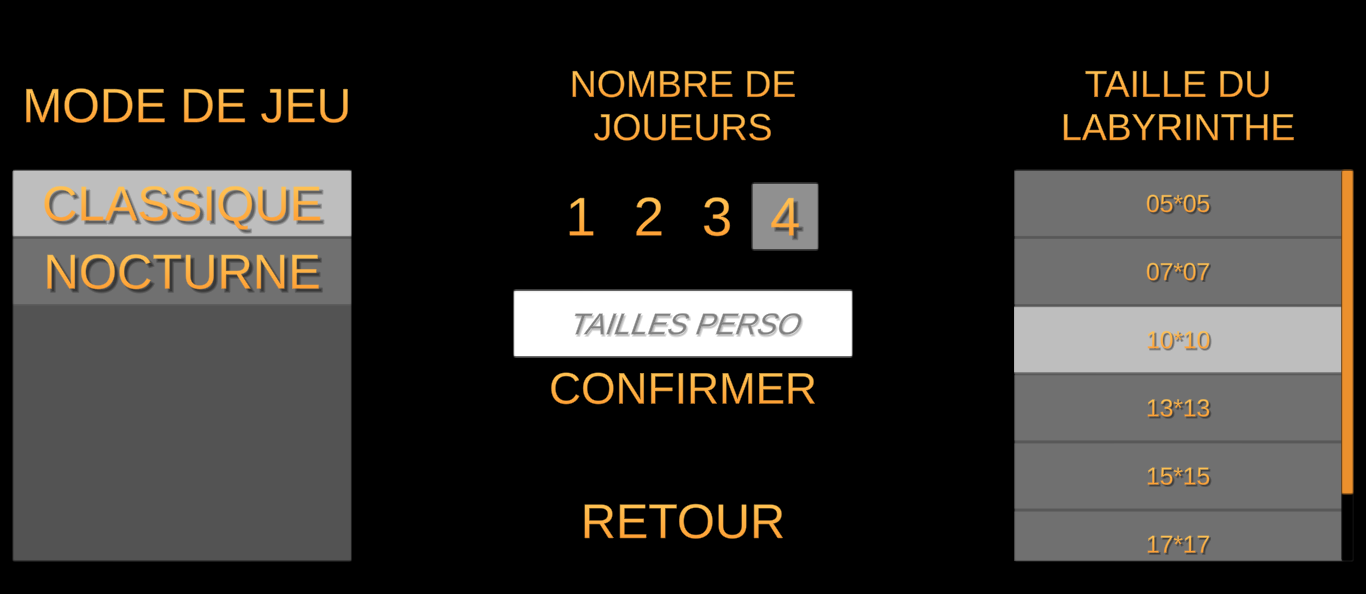
\includegraphics[width=0.8\textwidth]{Menu2.png}
    \caption{Menu pour les paramètres de la partie}
    \label{Menu pour les paramètres de la partie}
\end{figure}


\paragraph{Menu pour commencer la partie}

Ce menu a la particuliarité d'être différend en fonction de notre rôle dans la partie. Si on est l'hôte de la salle, alors le bouton en bas à gauche est "Commencer" permettant de débuter la partie, et sinon il est nommé "Prêt" qui permet de savoir si chacun des joueurs est prêt à commencer la partie comme montré sur les Figures 3 et 4. D'ailleurs à droite, on peut voir la liste des joueurs avec leur pseudonyme et leur rôle. A nôter que l'actualisation des statuts des joueurs est quasiment instantané et que le bouton "Prêt" change si on est prêt ou pas. Si on ne l'est pas il sera renommé "Non Prêt". L'hôte ne peut commencer la partie que si chacun des joueurs, et chacun des joueurs entre dans la salle avec un statut "Non Prêt". Dès que le nombre de joueurs attendus correspond au nombre de joueurs dans la salle et que tous les joueurs sont prêts, l'hôte peut débuter la partie. Lorsque la partie commence, la salle n'est plus accésible ni visible. En dehors de ça, peu importe notre rôle, on peut décider à tout moment de quitter la salle en appuyant sur le bouton éponyme. Si l'on est hôte, tous les joueurs de la salle sont transportés dans le menu pour créer la salle. De plus, des protections ont été mises de manière à ce que même si, par exemple, l'hôte viendrait à cliquer sur le bouton "	Commencer" alors que tous les joueurs ne sont pas prêts, la partie ne débutera pas.

\newpage
\begin{figure}[!ht]
    \centering
    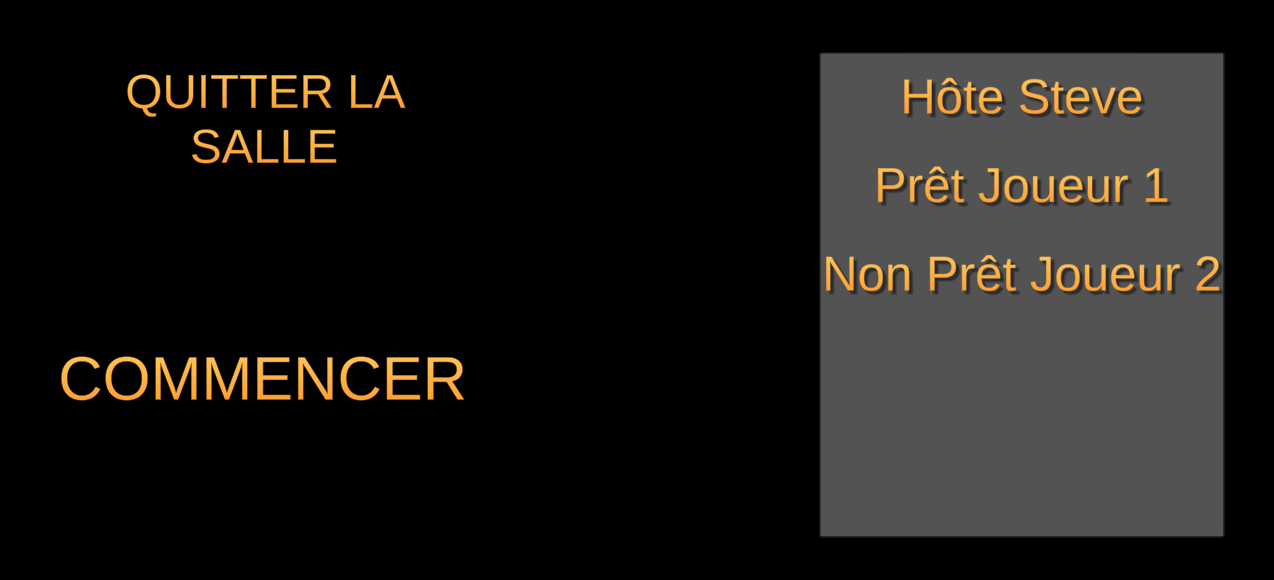
\includegraphics[width=0.8\textwidth]{Menu31.png}
    \caption{Menu lorsqu'on est hôte}
    \label{Menu lorsqu'on est hôte}
\end{figure}



\begin{figure}[!ht]
    \centering
    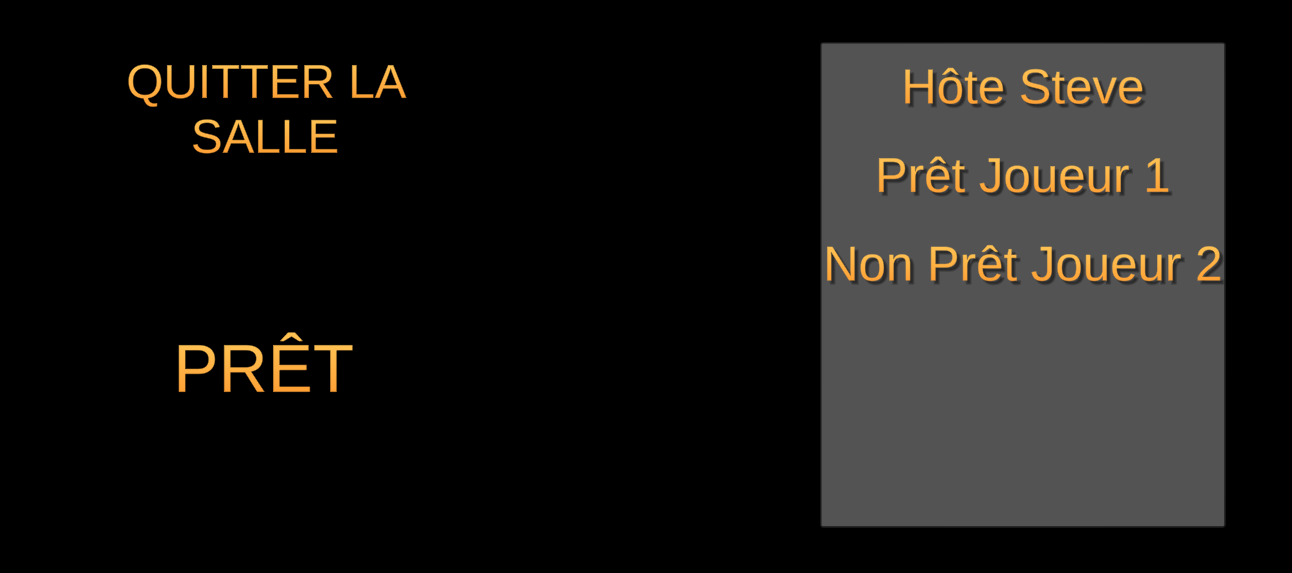
\includegraphics[width=0.8\textwidth]{Menu32.png}
    \caption{Menu lorsqu'on n'est pas hôte}
    \label{Menu lorsqu'on n'est pas hôte}
\end{figure}


\paragraph{Interface}
blablabla
\subsection{Gameplay}
blablabla
\subsubsection{Joueur}
%%%%%%%%%%%%%%%%%%%%%% Celian %%%%%%%%%%%%%%%%%%%%%%%%%%%%%%
blablabla
\subsubsection{Power-Up}
%%%%%%%%%%%%%%%%%%%%%% Léandre %%%%%%%%%%%%%%%%%%%%%%%%%%%%%%
blablabla
\subsection{Labyrinthe}
blablabla
%%%%%%%%%%%%%%%%%%%%%% Steve%%%%%%%%%%%%%%%%%%%%%%%%%%%%%%
\subsection{Réseau}
blablabla
\subsection{Site Web}
blablabla
%%%%%%%%%%%%%%%%%%%%%% Yann %%%%%%%%%%%%%%%%%%%%%%%%%%%%%%
\subsection{Sons et musiques}
blablabla
\subsubsection{Sons}
blablabla
\subsubsection{Musiques}
%%%%%%%%%%%%%%%%%%%%%% Léandre %%%%%%%%%%%%%%%%%%%%%%%%%%%%%%
%%%%%%%%%%%%%%%%%%%%%% Celian %%%%%%%%%%%%%%%%%%%%%%%%%%%%%%

\newpage
\section{Réalisations}
blablabla
\subsection{Nos joies}
blablabla
\subsection{Nos peines}
blablabla
\newpage
\section{Conclusion}

%%%%%%%%%%%%%%%%%%%%%%%%%%%%%% TODO : Mettre a jour

\emph{If you knew time as well as I do, you would play Deadly Science.}


\end{document}



